
\chapter{Appendix}
\begin{appendices}
    \section{Admin Interface and Backend Management}
    The following appendix provides insights into the administrative capabilities, security features, and monitoring tools used in ft\_transcendence.

    \begin{figure}[H]
        \centering
        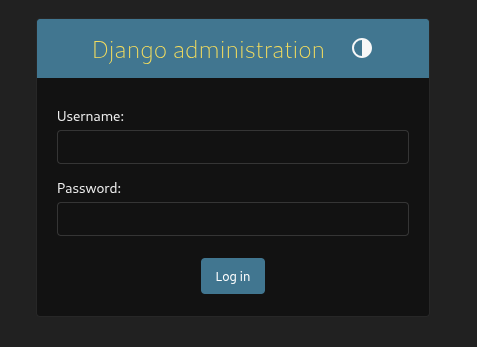
\includegraphics[width=0.7\linewidth]{Figures/appendix/DjangoAdminLogin.png}
        \caption*{Admin Login Interface}
        \label{fig:django-admin-login}
    \end{figure}
    
    \noindent Secure administrative access point for authorized system administrators. This interface requires valid admin credentials and supports the same security features as the main application.

    \begin{figure}[H]
        \centering
        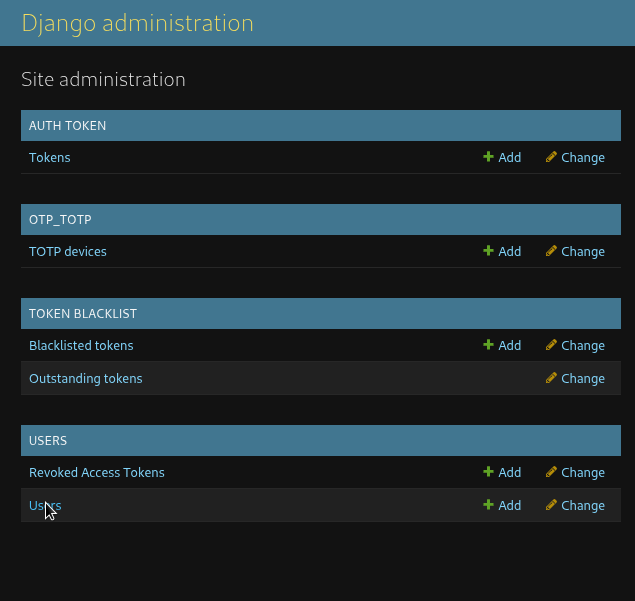
\includegraphics[width=0.75\linewidth]{Figures/appendix/DjangoAdminHome.png}
        \caption*{Admin Dashboard Panel}
        \label{fig:django-admin-home}
    \end{figure}
    
    \noindent Central control panel for system administration, providing access to all database models and data management tools. This interface allows authorized administrators to manage users, games, tournaments, and other application components.

    \begin{figure}[H]
        \centering
        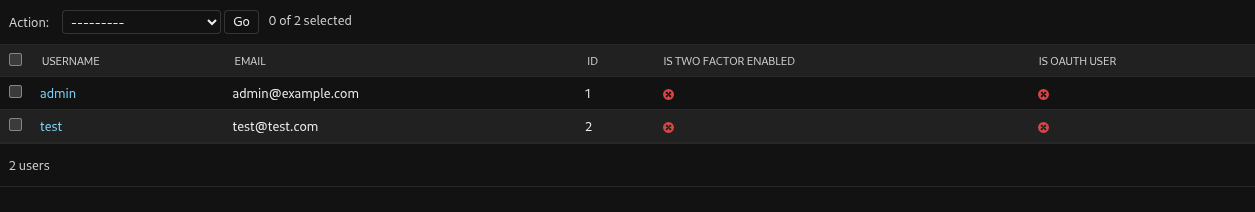
\includegraphics[width=0.65\linewidth]{Figures/appendix/ListedUsers.png}
        \caption*{User Management View}
        \label{fig:listed-users}
    \end{figure}
    
    \noindent Administrative view of all registered users with basic information and management controls. This tool allows administrators to monitor user accounts and take administrative actions when necessary.

    \begin{figure}[H]
        \centering
        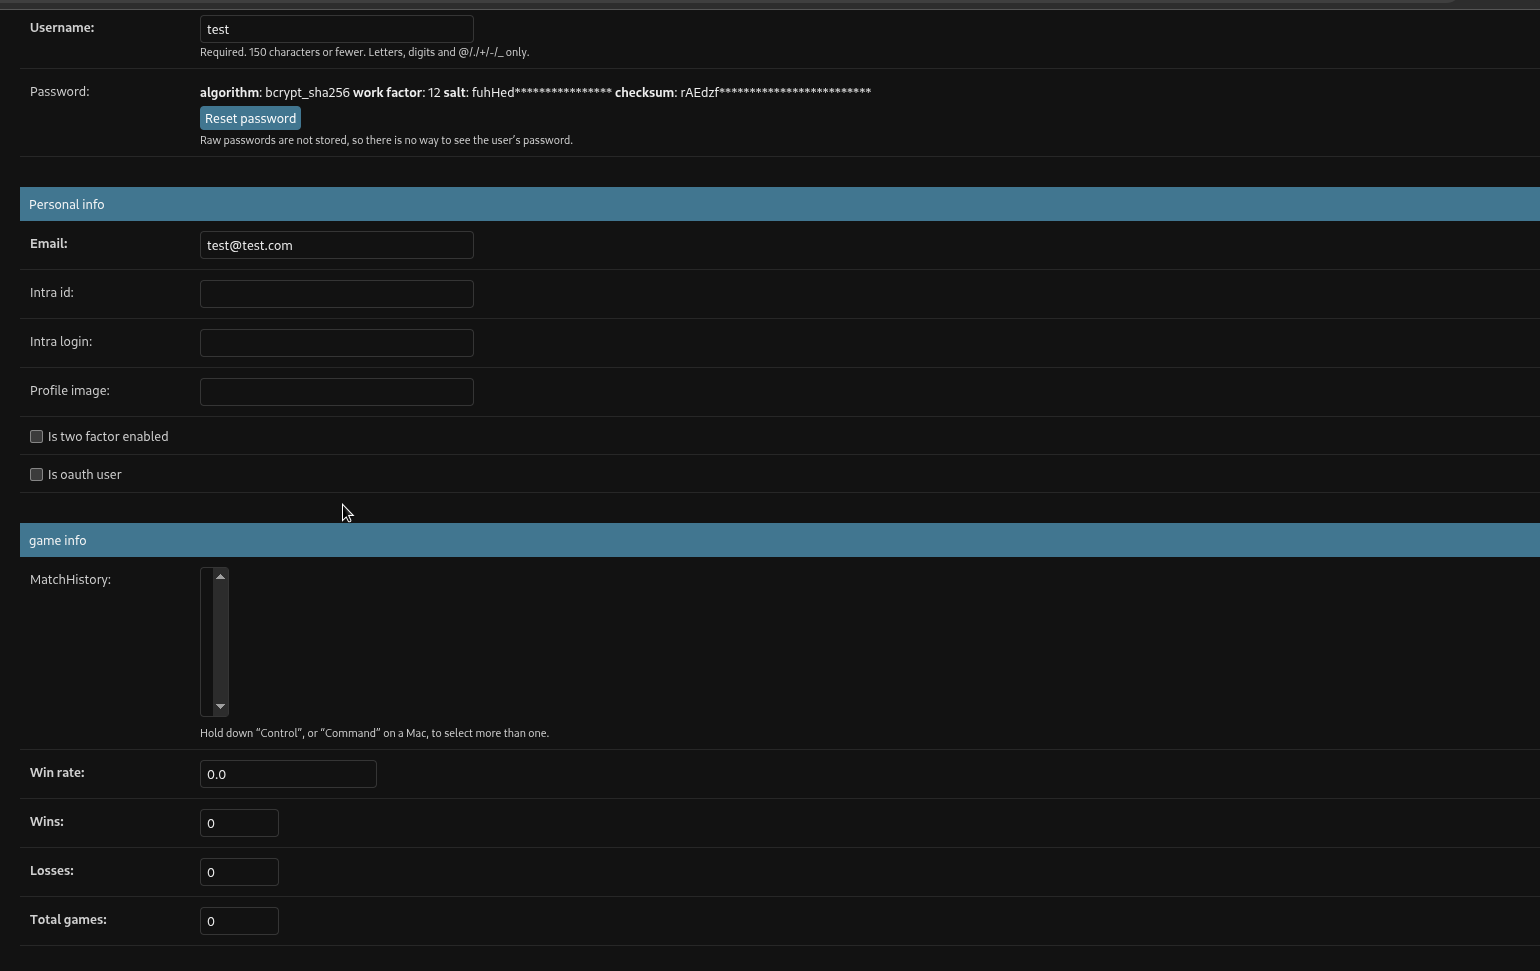
\includegraphics[width=0.7\linewidth]{Figures/appendix/UserDetailsInDjangoAdmin.png}
        \caption*{User Details Panel}
        \label{fig:user-details}
    \end{figure}
    
    \noindent Comprehensive view of individual user data including registration details, account settings, and platform activities. This interface provides administrators with detailed information about specific user accounts.

    \begin{figure}[H]
        \centering
        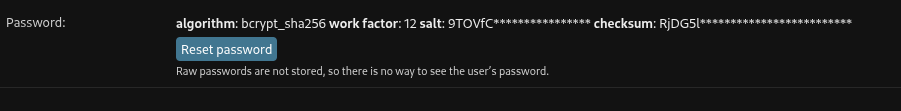
\includegraphics[width=0.6\linewidth]{Figures/appendix/PassewordIsHashed.png}
        \caption*{Password Hashing System}
        \label{fig:password-hashing}
    \end{figure}
    
    \noindent Visualization of the secure password hashing system that protects user credentials. Passwords are never stored in plain text but instead securely hashed in accordance with modern security standards to prevent unauthorized access.

    \section{Monitoring and Logging System}
    The application includes robust monitoring and logging capabilities to ensure system health and troubleshooting capabilities.

    \begin{figure}[H]
        \centering
        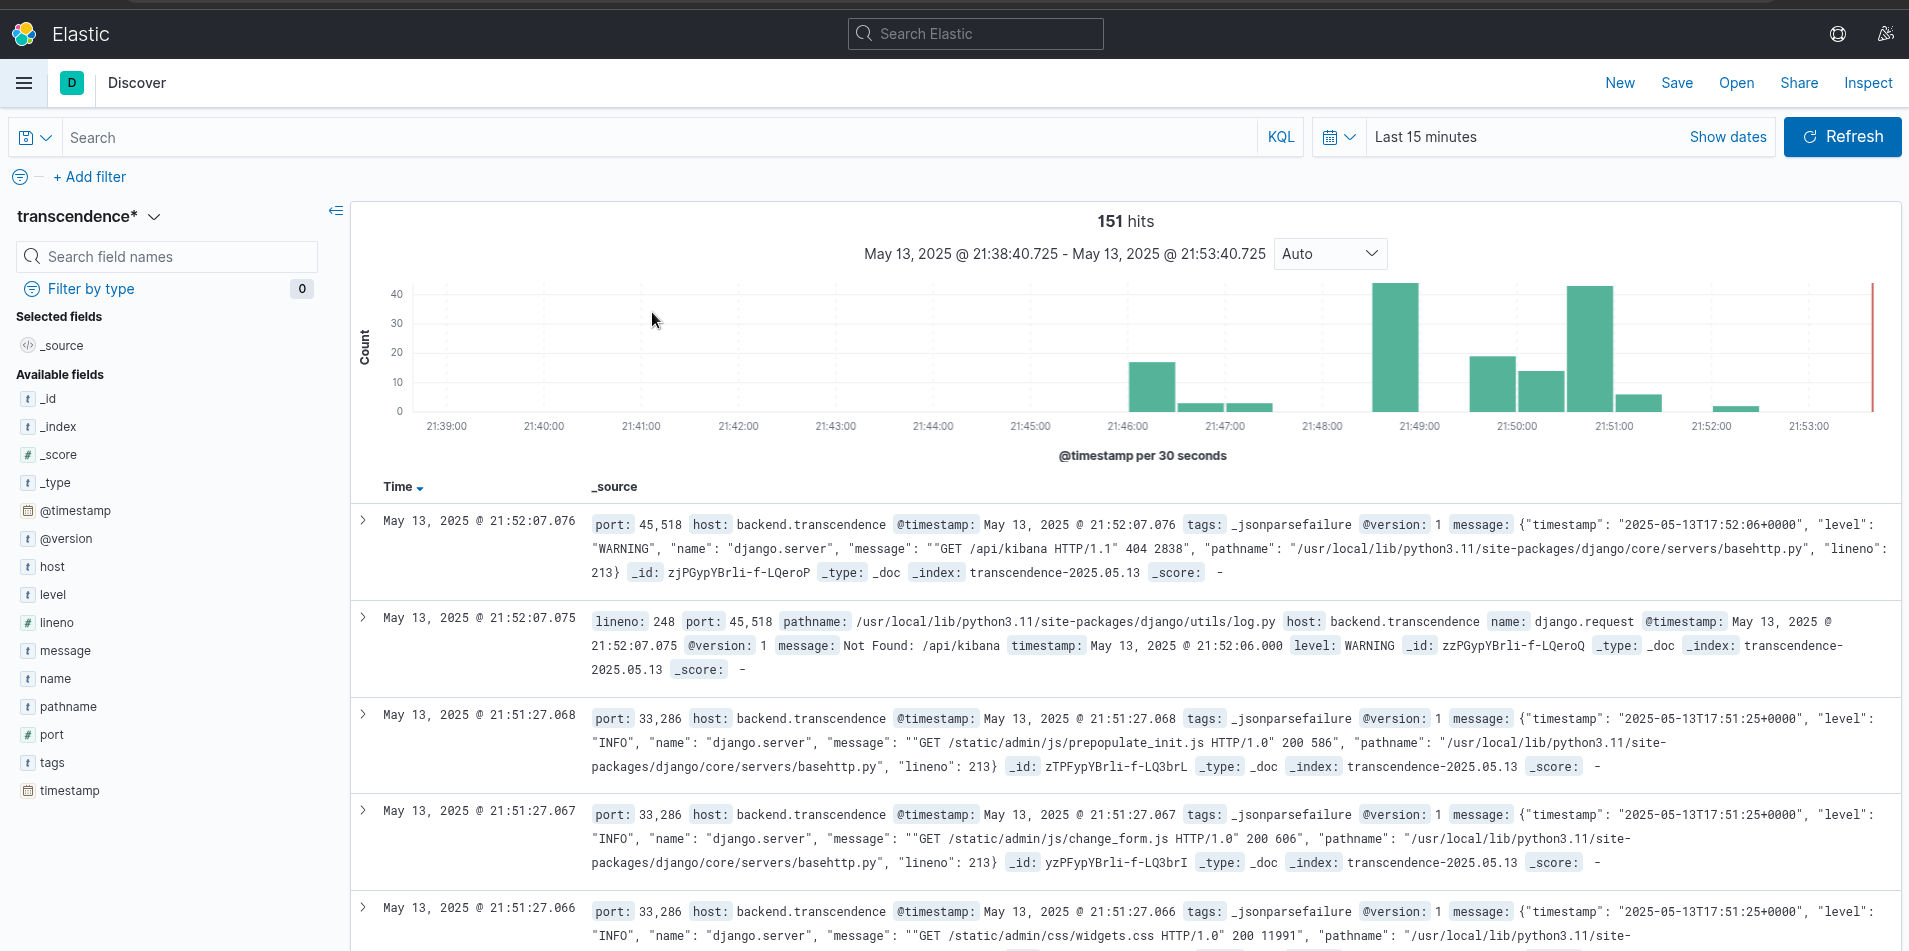
\includegraphics[width=0.75\linewidth]{Figures/appendix/ElasticBackendLogs.png}
        \caption*{Backend Logging System}
        \label{fig:elastic-logs}
    \end{figure}
    
    \noindent Real-time monitoring of application events and error tracking. This centralized logging system captures detailed information about system operations, helping developers identify and resolve issues quickly.

    \begin{figure}[H]
        \centering
        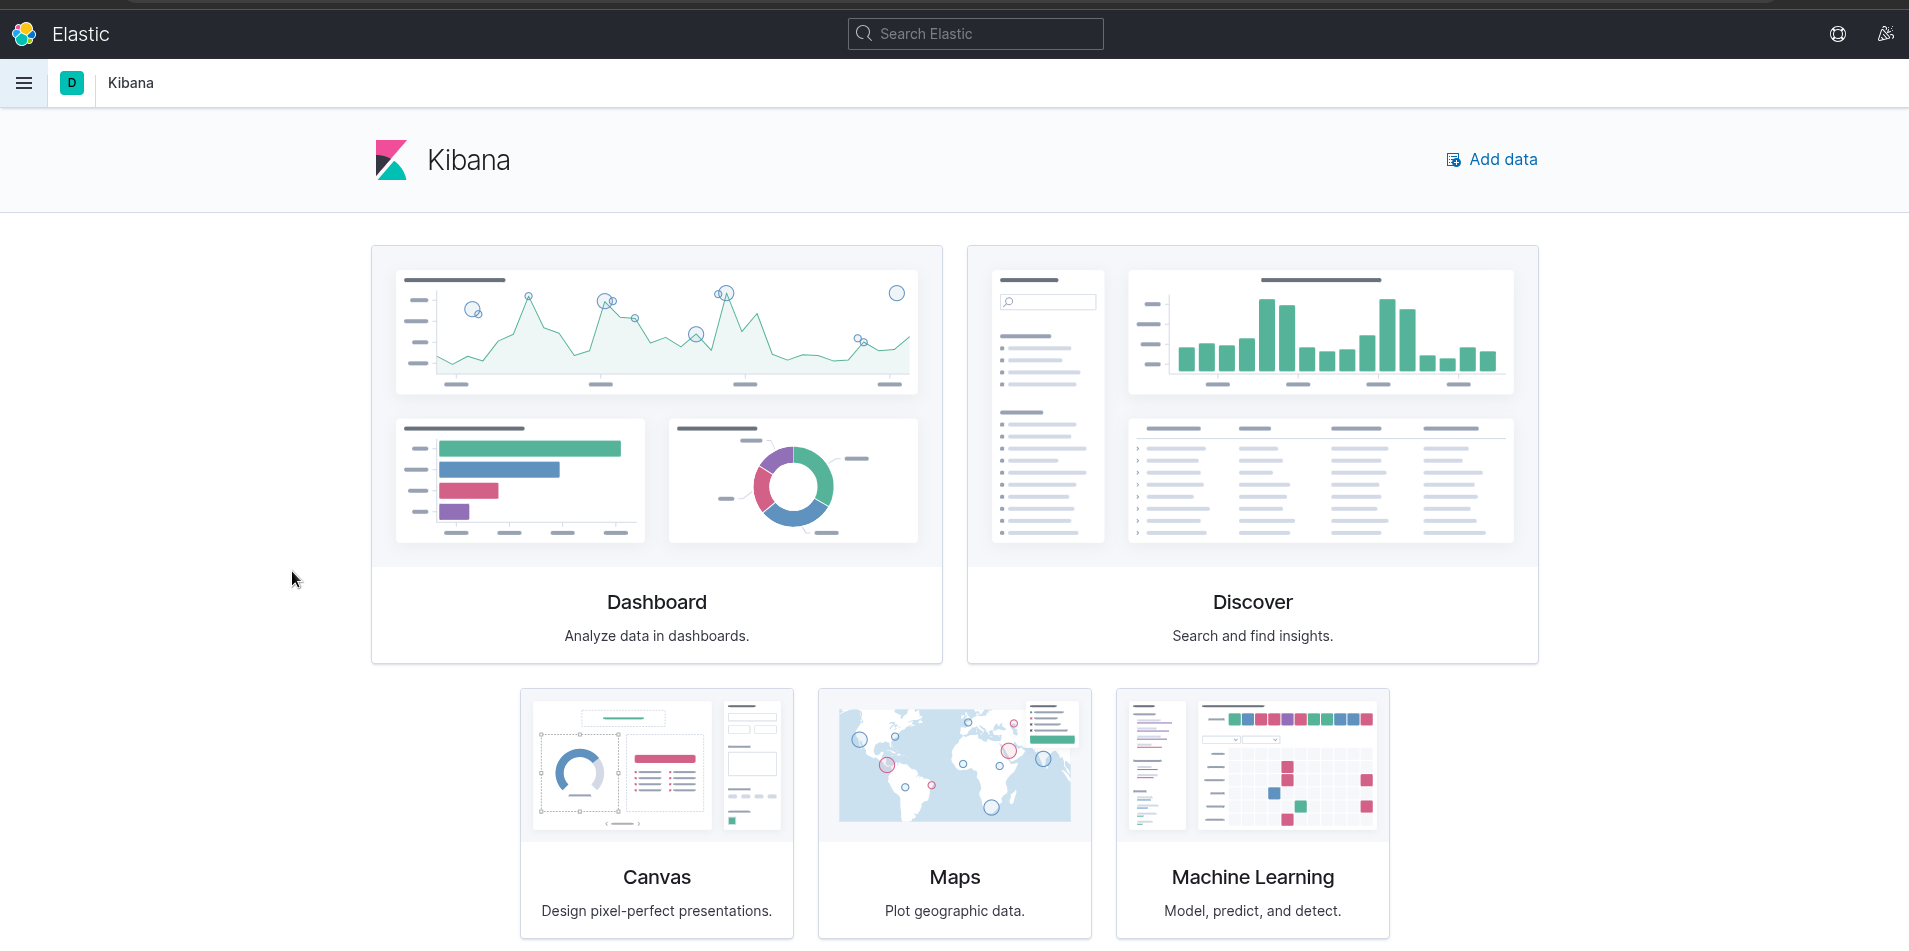
\includegraphics[width=0.7\linewidth]{Figures/appendix/KibanaHome.png}
        \caption*{Monitoring Dashboard Interface}
        \label{fig:kibana-dashboard}
    \end{figure}
    
    \noindent Advanced visualization interface for log analysis and system performance monitoring. This tool provides customizable charts and graphs to help administrators understand system behavior and identify trends or anomalies.

\end{appendices}